\documentclass[a4paper,11pt]{article}
\title{Search Engine Optimisation and Syndicating Dynamic Content}
\author{Tom Taylor -- 13015452}
\renewcommand\thesubsection{\roman{subsection}}
\usepackage{hyperref}
\usepackage{graphicx}
\usepackage[margin=0.5in]{geometry}
\date{15th October 2015}

\begin{document}
\maketitle
\section{Techiques used for Search Engine Optimisation}
\subsection{Title}
This is the first thing seen by both crawlers indexing the page and visitors landing on the Search Engine Results Page (SERP). It should make sense but also contain some relevant keywords to optimise for search.

\subsection{Meta description}
Less important that the title and probably will not have much of an impact on the ranking, however it is often the first piece of content that will be seen by a user as it will be displayed on most SERPs.  An additional technique could once have been to include meta keywords, however it is widely publicised that these are now ignored by indexers due to the ease of their abuse.

\subsection{Webmaster Tools}
This is a free service offered by both Google and Bing (the two major search players at the moment).  It ensures that their crawlers are aware of your site and can sometimes offer tips on improving your rankings.

\subsection{Sitemap}
This is an XML file, often based on a schema from \url{http://www.sitemaps.org/schemas/sitemap/}, that while not likely to directly influence rankings on SERPs, it will allow crawlers that are aware of it (by submitting to their Webmaster Tools for example) to fully index your site.\\\url{https://support.google.com/webmasters/answer/70897?hl=en#1}

\subsection{HTTPS}
It is worth (at least with Google) offering an HTTPS version of your site (and ensuring their crawlers are aware of it).  Google have been quite public about their prefereneces for HTTPS over plain HTTP.  Unfortunately the HTTPS certificate used by Birkbeck DCS is signed with SHA-1 HMACs which Google publically shame however it is not documented whether this has a negative impact on rankings at this time.

\subsection{Links}
This is the basis of the page ranking algorithm.  This invlolves linking to and from page swith good reputation. In this instance the page was linked to from my own personal homepage (which has been indexed for a few years), my LinkedIn profile and from a page within Martin O'Sheas university site.  It also contains many links out to reputable and authoirtative sites within its content.  These links must be natural though so as not to be considered spam.

\subsection{Formatting, Language and Content}
Clear language and so called prominence factors (sections, headings, lists etc) are also taken in to account by modern indexers.  There must also be what the indexers Natural Language Processors percieve to be actual relevent content.

\newpage

\section{Problems with aggregating dynamic content}

In the assignment, it was clearly hinted that we should use Javascript to syndicate RSS feeds from external sources.  The main problem with this from an SEO perspective is that the content is not stored in the retrieved page.  One possible solution for this would be for a server-side application (e.g. Rails, PHP etc) to pre-fetch the content from the RSS feeds and render the content as plain HTML in the page.
In the last few years it has come to light that Google is now able to execute client side Javascript and then re-read the DOM.

Another problem is stale content being indexed and therefore making the index irrelevent.  One solution for this is using submitted sitemaps and specifiying the frequency of change on the site/pages.  This is not guaranteed to be honoured by the crawlers but is considered a hint to the longivity of the validity of the content.

\section*{Links}

The rankings below were checked on \url{https://www.startpage.com}, an anonymous Google proxy.  By default, no location is passed to Google.  Use of startpage removes any preferences or distortions due to personalisation of results.

\begin{itemize}

  \item Homepage optimised for search term "Tom Taylor MSc")\\
  Ranked \#1 on October 10th 2015\\
  \url{https://www.dcs.bbk.ac.uk/~ttayl08}

  \item Page optimised for search term "search engine optimisation dynamic content"\\
  Ranked \#2 on October 10th 2015 \\
  \url{https://www.dcs.bbk.ac.uk/~ttayl08/search_dynamic.html}

  \item Syndicated dynamic content (News aggregator)\\
  \url{https://www.dcs.bbk.ac.uk/~ttaylo08/dynamic_content.html}

\end{itemize}

\begin{figure}[h]
  \centering
  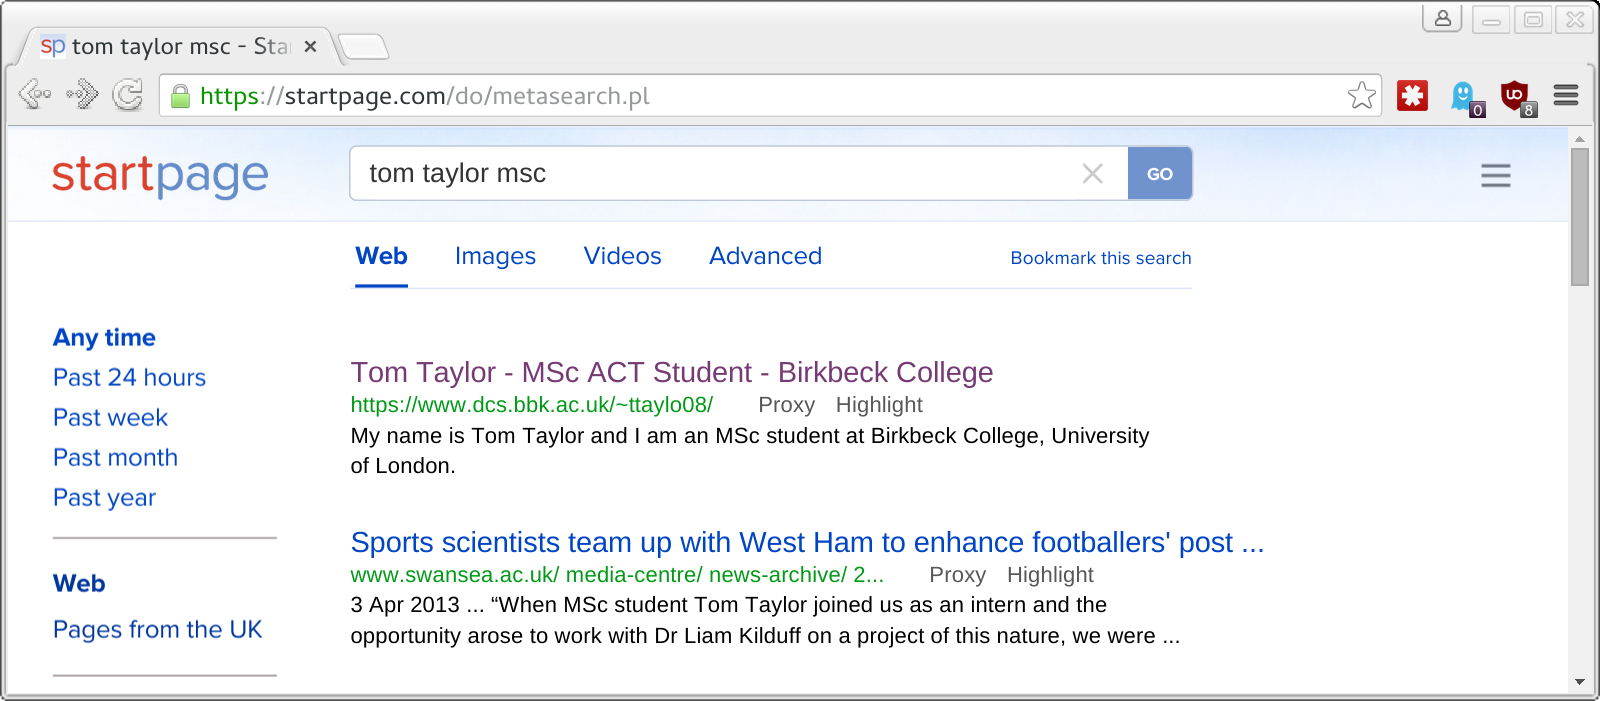
\includegraphics[height=5cm]{tom_taylor_msc.png}
  \caption{Search for "tom taylor msc"}
\end{figure}

\begin{figure}[h]
  \centering
  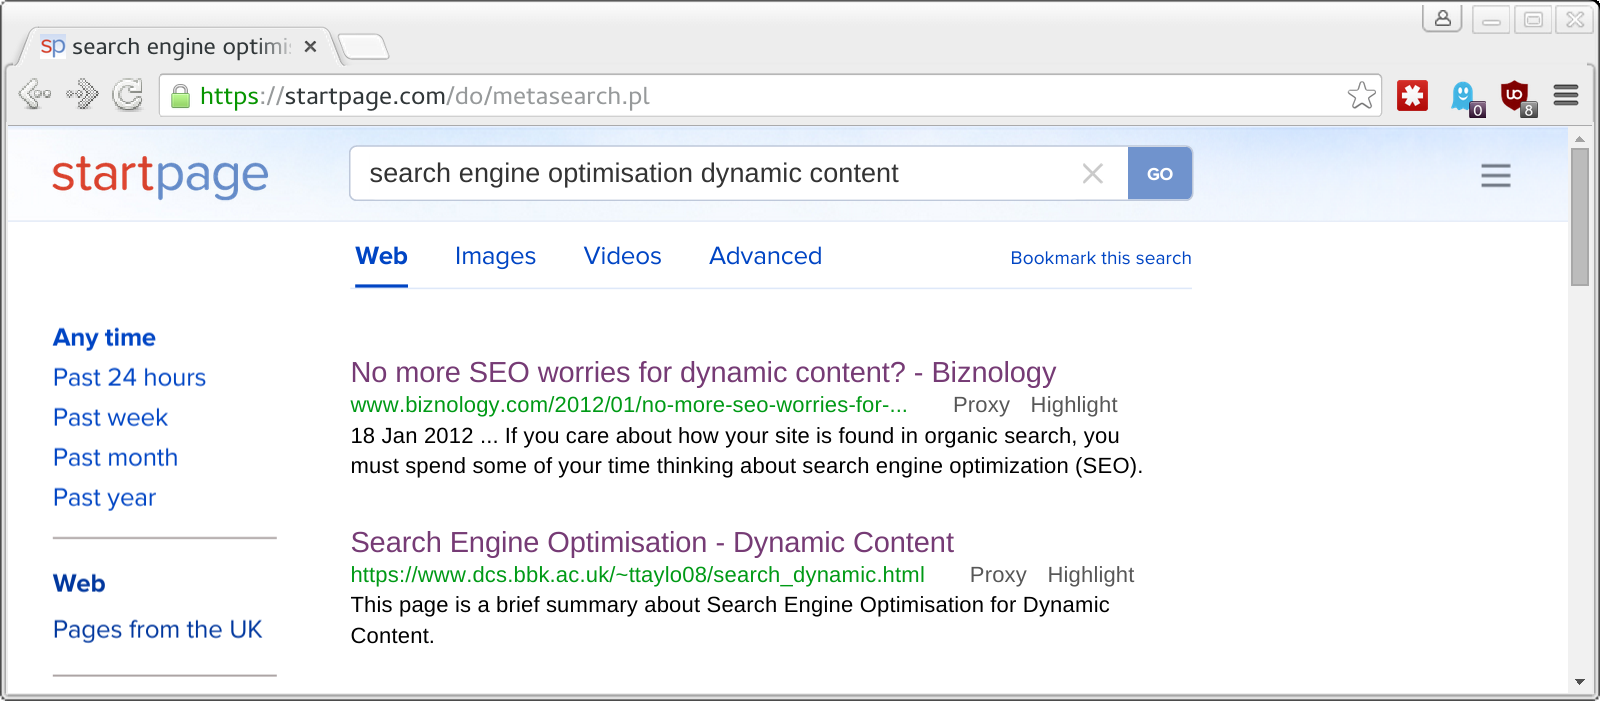
\includegraphics[height=5cm]{seo_dynamic.png}
  \caption{Search for "search engine optimisation dynamic content"}
\end{figure}


\end{document}
